% Create appendix with unnumbered section
%\section*{APPENDIX D - Phase Diagram}
\appendixsection{D}{Phase Diagram}
\setappendixlabel{D}

% Add appendix to toc at section level
\label{appendix:pfc-phase-diagram}
\subsection{Standard PFC Phase Diagram}

The PFC model superimposes a pattern-forming operator onto a Landau $\phi^4$ model for phase separation, enabling PFC to phase-separate between low-density and high-density regions, as well as between various crystalline patterns.  In the standard PFC model, a single length-scale given by $q_0$ enables three polymorphs of the PFC crystal - triangle, stripe, and hexagonal - in addition to the liquid or constant phase.
%
\begin{subequations}
\begin{align}
& F(n) = \int d\vec{r} \left[ \frac{1}{2}\beta n (\nabla^2 + {q_0}^2)^2 n + \frac{1}{2} \epsilon n^2 + \frac{1}{3} g n^3 + \frac{1}{4} n^4 \right], \label{eq-phase-diagram-std-pfc-energy} \\
& \partialt n(\pos, t) = \nabla^2 \left[ \beta (\nabla^2 + {q_0}^2)^2 n + \epsilon n + g n^2 + n^3 \right], \label{eq-phase-diagram-std-pfc-dndt}
\end{align}
\end{subequations}
%
For a particular set of model parameters $\beta, \epsilon,$ and $g$, phase selection is largely determined by the average system density $\mean{n}$, with phase transitions from liquid to triangle to stripe to honeycomb back to liquid as the average density is increased.

Simulations show a certain degree of sensitivity to initial conditions.  For example, an ensemble of systems initialized with randomly distributed density fluctuations around a given average density may settle into a mixture of two phases with slightly varying ratios between phases or a system initialized with a particular lattice structure may remain in that lattice structure rather than shifting into a lower-energy lattice structure or liquid phase.  There are two distinct drivers of this behavior.  The first is quasistatic states at unstable equilibriums.  For example, a system initialized with an identical density at every point will remain in the constant state indefinitely, even if a slight perturbation of this flat density landscape would give rise to a different equilibrium.  The second is the energy of phase boundaries, which must be overcome to transition from one phase to another.  However, the first driver can be overcome by imposing small perturbations on initial states, while the second driver can be quantified by running multiple simulations with varying initial density fields or adding stochastic noise to the time-evolution of the system.

To estimate the PFC phase diagram, Elder et al. used one-mode approximations of the triangle, stripe, and honeycomb lattices \cite{elder2002modeling} given by.
%
\begin{subequations}
\begin{align} \label{eqn-pfc-ansatze}
& n_t(\pos) = \mean{n} + A_T \sum_{j=1}^3 \left[ e^{i \mathbf{q}_j \cdot \pos} + \text{c.c.} \right], \\
& n_s(\pos) = \mean{n} + A_S \left[ e^{i \mathbf{q}_2 \cdot \pos} + \text{c.c.} \right], \\
& n_h(\pos) = \mean{n} + A_H \sum_{j=1}^3 \left[ e^{i \mathbf{q}_j \cdot \pos} + \text{c.c.} \right],
\end{align}
\end{subequations}
%
respectively, with $\mathbf{q}_{j=1,2,3} = \{q_{t,s,h}(-\sqrt{3}/2, -1/2), q_{t,s,h}(0, 1), q_{t,s,h}(\sqrt{3}/2, -1/2)\}$.  Substituting these states into Eq.~\ref{eq-phase-diagram-std-pfc-energy} and dividing by the unit cell area gives the mean energy density for each state in terms of the model parameters $\beta, \epsilon,$ and $g$, and the mean density $\mean{n}$, amplitude $A_{t, s, h}$, and length-scale $q_{t, s, h}$ as
%
\begin{subequations}
\begin{align}
f_T(\mean{n}, A_T, q_T) &= \frac{45}{2} A_T^{4} + 4 A_T^{3} g + 12 A_T^{3} n_{0} + 3 A_{t}^{2} \beta q_T^{4} - 6 A_{t}^{2} \beta q_T^{2} q_{0}^{2} + 3 A_{t}^{2} \beta q_{0}^{4} \nonumber \\
&\quad + 3 A_{t}^{2} \epsilon + 6 A_{t}^{2} g n_{0} + 9 A_{t}^{2} n_{0}^{2} + \frac{\beta n_{0}^{2} q_{0}^{4}}{2} + \frac{\epsilon n_{0}^{2}}{2} + \frac{g n_{0}^{3}}{3} + \frac{n_{0}^{4}}{4}, \\
f_S(\mean{n}, A_S, q_S) &= \frac{3}{2} A_S^{4} + A_S^{2} \beta q_S^{4} - 2 A_S^{2} \beta q_S^{2} q_{0}^{2} + A_S^{2} \beta q_{0}^{4} + A_S^{2} \epsilon + 2 A_S^{2} g n_{0} + 3 A_S^{2} n_{0}^{2} \nonumber \\
&\quad  + \frac{\beta n_{0}^{2} q_{0}^{4}}{2} + \frac{\epsilon n_{0}^{2}}{2} + \frac{g n_{0}^{3}}{3} + \frac{n_{0}^{4}}{4}, \\
f_H(\mean{n}, A_H, q_H) &= \frac{45}{2} A_H^{4} - 4 A_H^{3} g - 12 A_H^{3} n_{0} + 3 A_{t}^{2} \beta q_H^{4} - 6 A_{t}^{2} \beta q_H^{2} q_{0}^{2} + 3 A_{t}^{2} \beta q_{0}^{4} \nonumber \\
&\quad + 3 A_{t}^{2} \epsilon + 6 A_{t}^{2} g n_{0} + 9 A_{t}^{2} n_{0}^{2} + \frac{\beta n_{0}^{2} q_{0}^{4}}{2} + \frac{\epsilon n_{0}^{2}}{2} + \frac{g n_{0}^{3}}{3} + \frac{n_{0}^{4}}{4}.
\end{align}
\end{subequations}
%
These energy densities are minimized by $q_T = q_S = q_T = q_0$ and
%
\begin{subequations}
\begin{align}
A_T(\mean{n}) &= -\frac{g}{15} - \frac{\mean{n}}{5} + \frac{\sqrt{-15 \epsilon + g^2 - 24 g \mean{n} - 36 \mean{n}^2}}{15} \label{eqn-std-pfc-A-min-triangle} \\
A_S(\mean{n}) &= \frac{\sqrt{-3 \epsilon - 6 g \mean{n} - 9 \mean{n}^2}}{3},  \label{eqn-std-pfc-A-min-stripe}\\
A_H(\mean{n}) &= \frac{g}{15} + \frac{\mean{n}}{5} + \frac{\sqrt{-15 \epsilon + g^2 - 24 g \mean{n} - 36 \mean{n}^2}}{15}. \label{eqn-std-pfc-A-min-honeycomb}
\end{align}
\end{subequations}
%
Substituting back into the energy densities above gives
%
\begin{subequations}
\begin{align}
f_T(\mean{n}) &= - \frac{13}{500} \mean{n}^{4} + \left(- \frac{16 \omega}{125} - \frac{13 g}{375}\right) \mean{n}^{3} + \left(\frac{\beta q_{0}^{4}}{2} + \frac{7 \epsilon}{50} - \frac{16 \omega g}{125} - \frac{8 g^{2}}{125}\right) \mean{n}^{2} \nonumber \\
& \quad + \left(- \frac{4 \epsilon \omega}{75} - \frac{6 \epsilon g}{25} - \frac{28 \omega g^{2}}{1125} + \frac{44 g^{3}}{1125}\right) \mean{n} - \frac{\epsilon^{2}}{10} - \frac{4 \epsilon \omega g}{225} + \frac{2 \epsilon g^{2}}{75} + \frac{4 \omega g^{3}}{3375} - \frac{4 g^{4}}{3375}, \nonumber \\
& \quad \omega = \sqrt{-15 \epsilon + g^2 - 24 g \mean{n} -36 \mean{n}^2} \\
%
f_S(\mean{n}) &= - \frac{5}{4} \mean{n}^4 - \frac{5 g}{3} \mean{n}^3 + \left( \frac{\beta q_0^4}{2} - \frac{\epsilon}{2} - \frac{2 g^2}{3} \right) \mean{n}^2 - \frac{2 \epsilon g}{3} \mean{n} - \frac{\epsilon^2}{6}, \\
%
f_H(\mean{n}) &= - \frac{13}{500} \mean{n}^{4} + \left(\frac{16 \omega}{125} - \frac{13 g}{375}\right) \mean{n}^{3} + \left(\frac{\beta q_{0}^{4}}{2} + \frac{7 \epsilon}{50} + \frac{16 \omega g}{125} - \frac{8 g^{2}}{125}\right) \mean{n}^{2} \nonumber \\
& \quad + \left(\frac{4 \epsilon \omega}{75} - \frac{6 \epsilon g}{25} + \frac{28 \omega g^{2}}{1125} + \frac{44 g^{3}}{1125}\right) \mean{n} - \frac{\epsilon^{2}}{10} + \frac{4 \epsilon \omega g}{225} + \frac{2 \epsilon g^{2}}{75} - \frac{4 \omega g^{3}}{3375} - \frac{4 g^{4}}{3375}, \nonumber \\
& \quad \omega = \sqrt{-15 \epsilon + g^2 - 24 g \mean{n} -36 \mean{n}^2}.
\end{align}
\end{subequations}
%
The density in the liquid region where $n = \mean{n}$ is simply
\begin{equation}
f_L(\mean{n}) = \frac{1}{4} \mean{n}^4 + \frac{g}{3} \mean{n}^3 + \left( \frac{\beta q_0^4}{2} + \frac{\epsilon}{2} \right) \mean{n}^2
\end{equation}
Then, for a given set of model parameters $\beta, \epsilon,$ and $g$, the phase for a given system's average density is determined by the phase corresponding to the minimum energy density among $f_T, f_S, f_H,$ and $f_L$.  Fig.~\ref{fig:free_energy_vs_avg_density} shows these functions plotted for a given set of model parameters over a range of densities.  The energy in this figure is minimized by the liquid phase at low density, transitions to the triangle phase around $\mean{n} \sim -0.55$, then to stripe phase around $\mean{n} \sim -0.19$, followed by honeycomb around $\mean{n} \sim 0.19$, and finally back to liquid phase around $\mean{n} \sim 0.55$.  Due to the sign of the radicals in the minimum amplitudes, energy densities of the triangular, stripe, and honeycomb phases are calculable over at most a finite range of densities for a given value of $\epsilon$ and $g$.  With $g=0$, no valid amplitudes can be calculated for $\epsilon > 0$ and at $\epsilon = 0$, the radicals are only valid for $\mean{n} = 0$.  Then for $g=0$ the values $\epsilon^* = 0$ and $\mean{n}^*$ are the \textit{critical} temperature and density.
%
\begin{figure}[!htbp]
    \centering
    \begin{subfigure}[t]{0.85\linewidth}
        \centering
        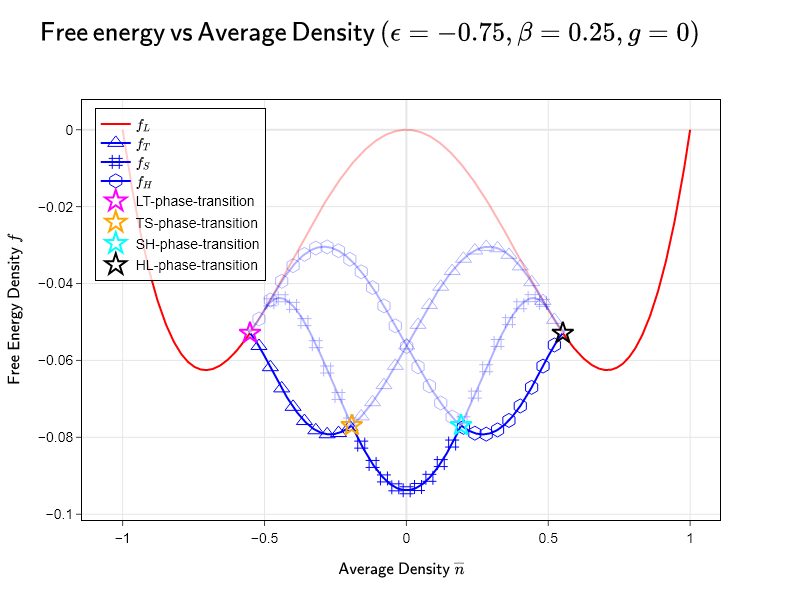
\includegraphics[width=\linewidth]{fig/fig-free_energy_vs_avg_density.png}
    \end{subfigure}
    \caption{Plots of energy densities $f_L, f_T, f_S,$ and $f_H$ with model parameters $\beta = 0.25, \epsilon = -0.75$ and $g = 0$.  The lowest energy for a given average density $\mean{n}$ is indicated by full line weight.  The transitions between densities are marked with stars. }
    \label{fig:free_energy_vs_avg_density}
\end{figure}
%

For any model parameters $\beta$ and $g$, a phase diagram can be constructed by varying $\epsilon$ and $\mean{n}$ and determining the phase whose energy density is minimal in that region of the parameter space. Inspection of the free energy equations demonstrates that the phase and critical points are independent of the $\beta$ model parameter, as all four energy densities contain the identical $\beta q_0^4/2$ term and no other factors of $\beta$.  The critical values of $\epsilon^*$ and $\mean{n}^*$ can be determined by simultaneously setting the expressions under the radicals in the amplitudes $A_T$ and $A_S$ to zero (the radicals in $A_T$ and $A_H$ are identical), giving
%

\begin{equation}
\epsilon^*(g) = \frac{g^2}{3}, \quad \mean{n}^*(g) = \frac{g}{3}.
\end{equation}
%
An example of a phase diagram for $g=0$ is given in Fig.~$\ref{fig:std-phase-diagram-app}$ where the transitions from liquid to triangle (LT), triangle to stripe (TS), stripe to honeycomb (SH), and honeycomb to liquid (HL) are indicated along with the critical point at $\mean{n}^* = 0$ and at $\epsilon^* = 0$ marked with a red x.
%
\begin{figure}[!htbp]
    \centering
    \begin{subfigure}[t]{0.85\linewidth}
        \centering
        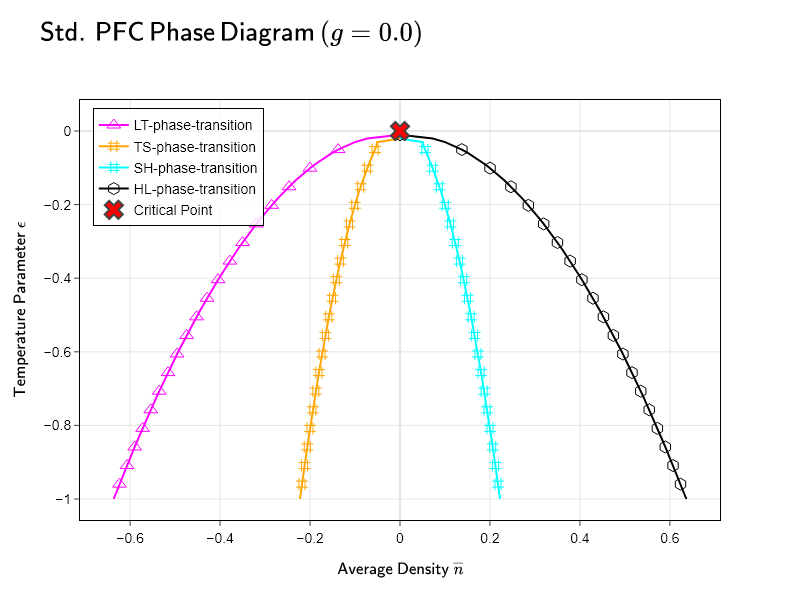
\includegraphics[width=\linewidth]{fig/fig-std-phase-diagram.png}
    \end{subfigure}
    \caption{Std. PFC Phase Diagram: The calculated phase transitions from liquid to triangle (LT), triangle to stripe (TS), stripe to honeycomb (SH), and honeycomb back to liquid (HL) are plotted for a range of average densities $\mean{n}$ and temperatures $\epsilon$.  The critical point $(\mean{n}^*, \epsilon^*)$ is marked with a red x.  At temperatures above $\epsilon^*$, no phase transitions occur and the system will always settle to a homogeneous state at any density.}
    \label{fig:std-phase-diagram-app}
\end{figure}
%
\subsection{Log PFC Phase Diagram}
In the log PFC model, the phase diagram cannot be obtained analytically, and numeric methods must be employed.  However, the general process is identical to the method outlined above for the standard PFC model.  In particular, the one-mode approximations given in Eq.~\ref{eqn-pfc-ansatze} are used with the log PFC energy functional to calculate energy densities by numeric integration as a function of amplitudes $A_T, A_S,$ and $A_H$ for a given set of model parameters $\beta, \epsilon,$ and $g$ at a particular mean density $\mean{\phi}$. For a given set of parameters, the corresponding amplitudes that minimize each free energy can be determined as a function of the system's mean density $\mean{\phi}$ by varying the amplitude over an appropriate range (in log PFC this range is limited by the positive-definite requirement of the log PFC density $\phi$).  Then, using these amplitudes, the values of $f_T, f_S,$ and $f_H$ can be calculated as functions of $\mean{\phi}$ and an appropriate phase diagram constructed by interrogating the transitions over a range of densities $\mean{\phi}$ and temperatures $\epsilon$.  The critical point can be estimated as the maximum temperature where the stripe phase energy density is minimal with amplitude $A_S > 0$ at any density $\mean{\phi}$.

The conversion of model parameters between models $\{\beta^S, \epsilon^S, g^S, n\} \leftrightarrow \{\beta^L, \epsilon^L, g^L, \phi\}$ calculated in Appendix \ref{appendix:pfc-rescaling} can help constrain the parameter space in the log PFC model over which the calculations described must be performed.  For example, the critical point for $g^S = 0$ at $\mean{n}^{*} = 0, \epsilon^{S*}=0 \leftrightarrow \mean{\phi}^*= 1, \epsilon^{L*} = 1$ at $g^L = -2.5$, and the overall log PFC phase diagram at $g^L=-2.5$ presented in Fig.~\ref{fig:log-phase-diagram-app} has a similar overall shape to the standard PFC phase diagram at $g^S=0$ presented in Fig.~\ref{fig:std-phase-diagram-app}.  The positive-definite constraint on $\phi$ tends to distort the behavior of the model, particularly as $\phi \rightarrow 0$.  This distortion is most noticeable along the (TS) phase boundary, where at low temperature $\epsilon$, the log PFC model shows the density of this transition reaching a minimum density or even increasing with lower temperature, whereas in the standard PFC model, the (TS) transition density decreases with temperature.
%
\begin{figure}[!htbp]
    \centering
    \begin{subfigure}[t]{0.85\linewidth}
        \centering
        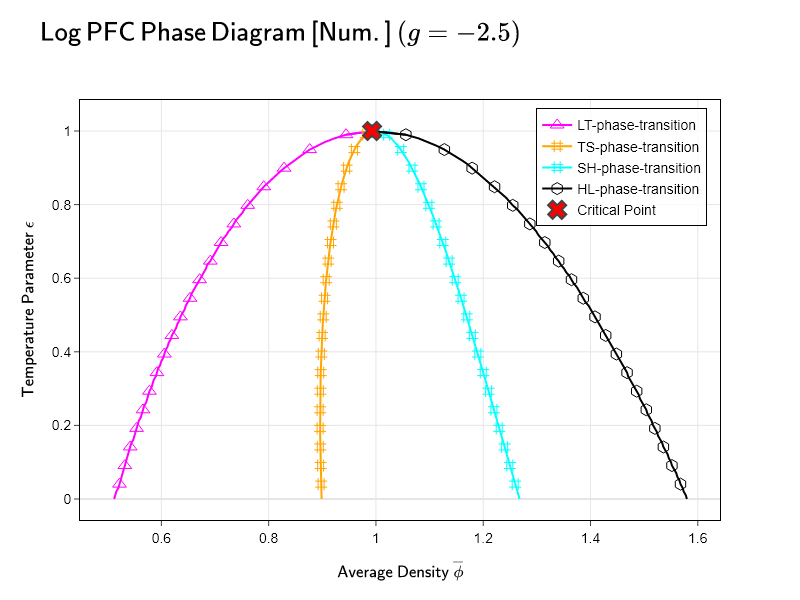
\includegraphics[width=\linewidth]{fig/fig-log-phase-diagram.png}
    \end{subfigure}
    \caption{Log PFC Phase Diagram: The calculated phase transitions from liquid to triangle (LT), triangle to stripe (TS), stripe to honeycomb (SH), and honeycomb back to liquid (HL) are plotted for a range of average densities $\mean{n}$ and temperatures $\epsilon$.  The critical point $(\mean{n}^*, \epsilon^*)$ is marked with a red x.  At temperatures above $\epsilon^*$, no phase transitions occur and the system will always settle to a homogeneous state at any density.}
    \label{fig:log-phase-diagram-app}
\end{figure}
%